\thispagestyle{duongvaotoanhocnone}
\pagestyle{duongvaotoanhoc}
\everymath{\color{duongvaotoanhoc}}
\graphicspath{{../duongvaotoanhoc/pic/}}
%\blfootnote{$^1$\color{duongvaotoanhoc}Theo Quanta Magazine.}
%\blfootnote{$^2$\color{duongvaotoanhoc}Hà Nội.}
\begingroup
\AddToShipoutPicture*{\put(0,616){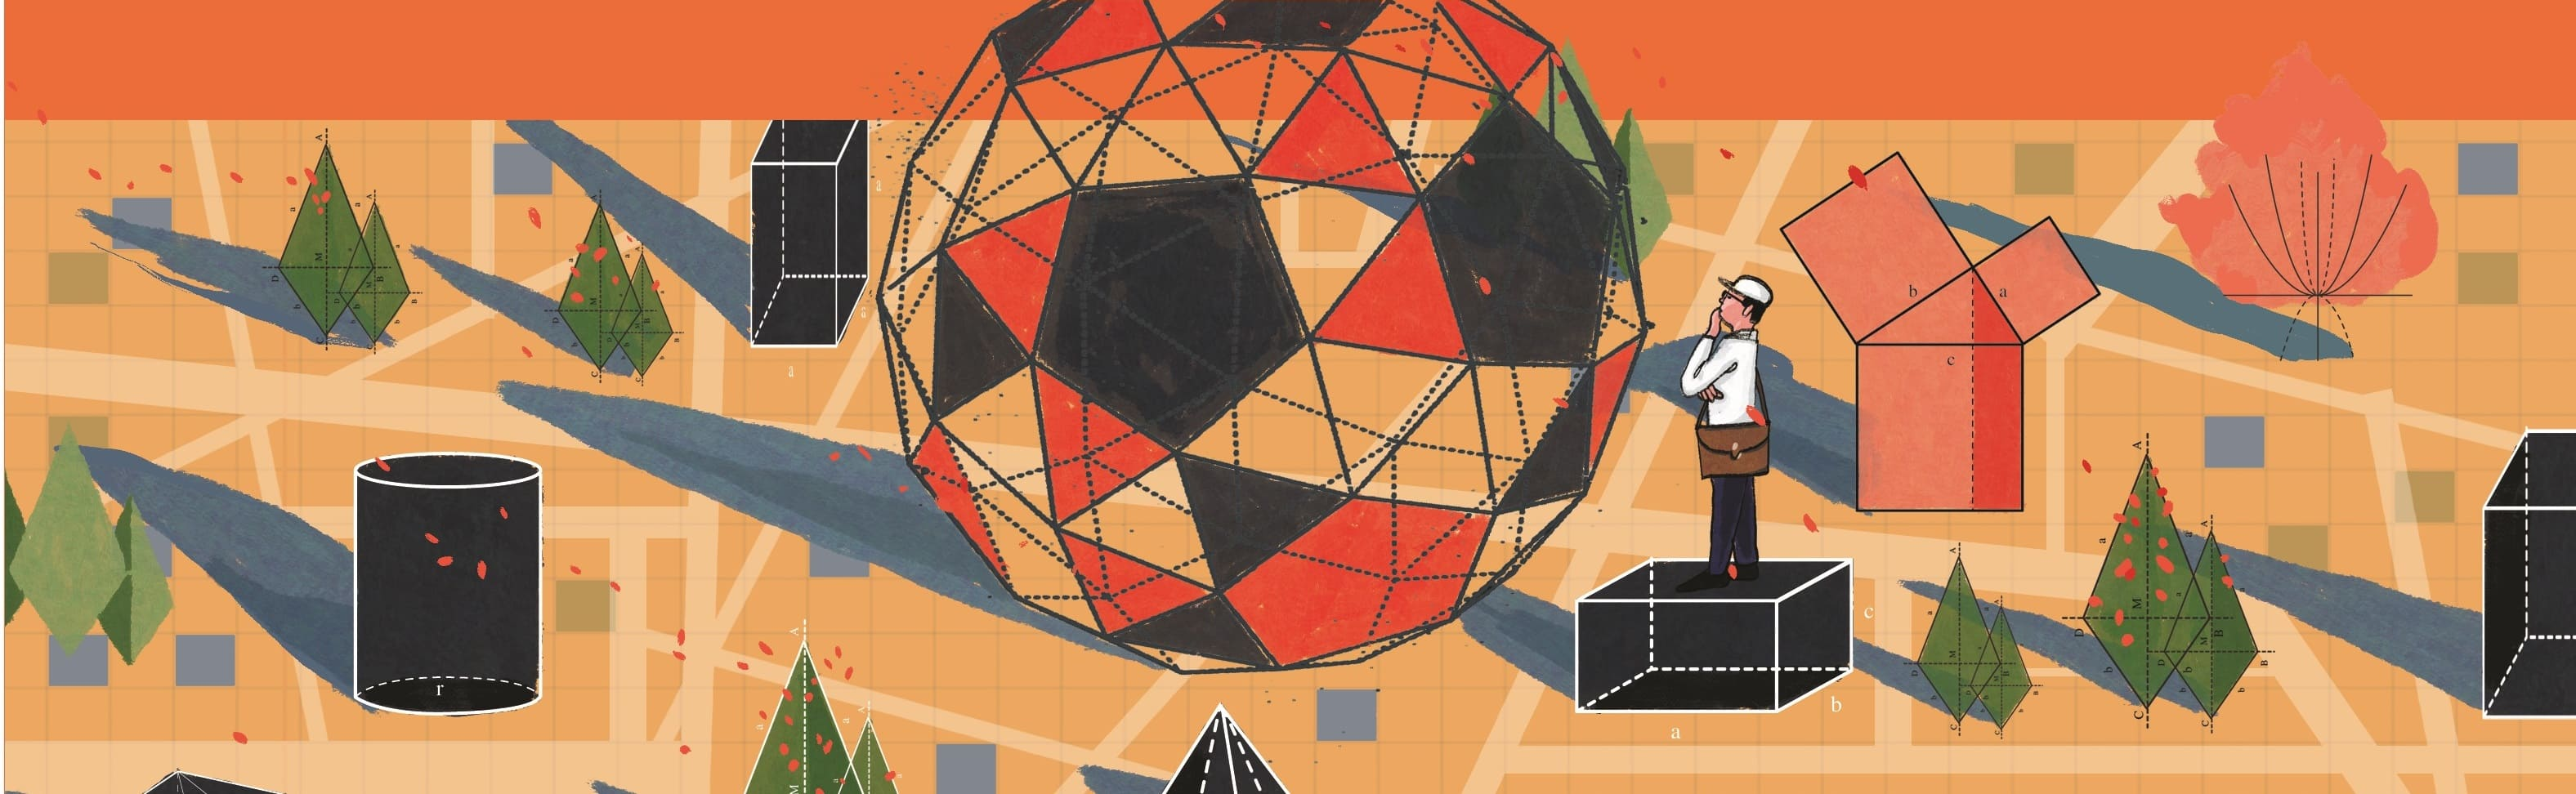
\includegraphics[width=19.3cm]{../bannerduongvao}}}
\AddToShipoutPicture*{\put(82,555){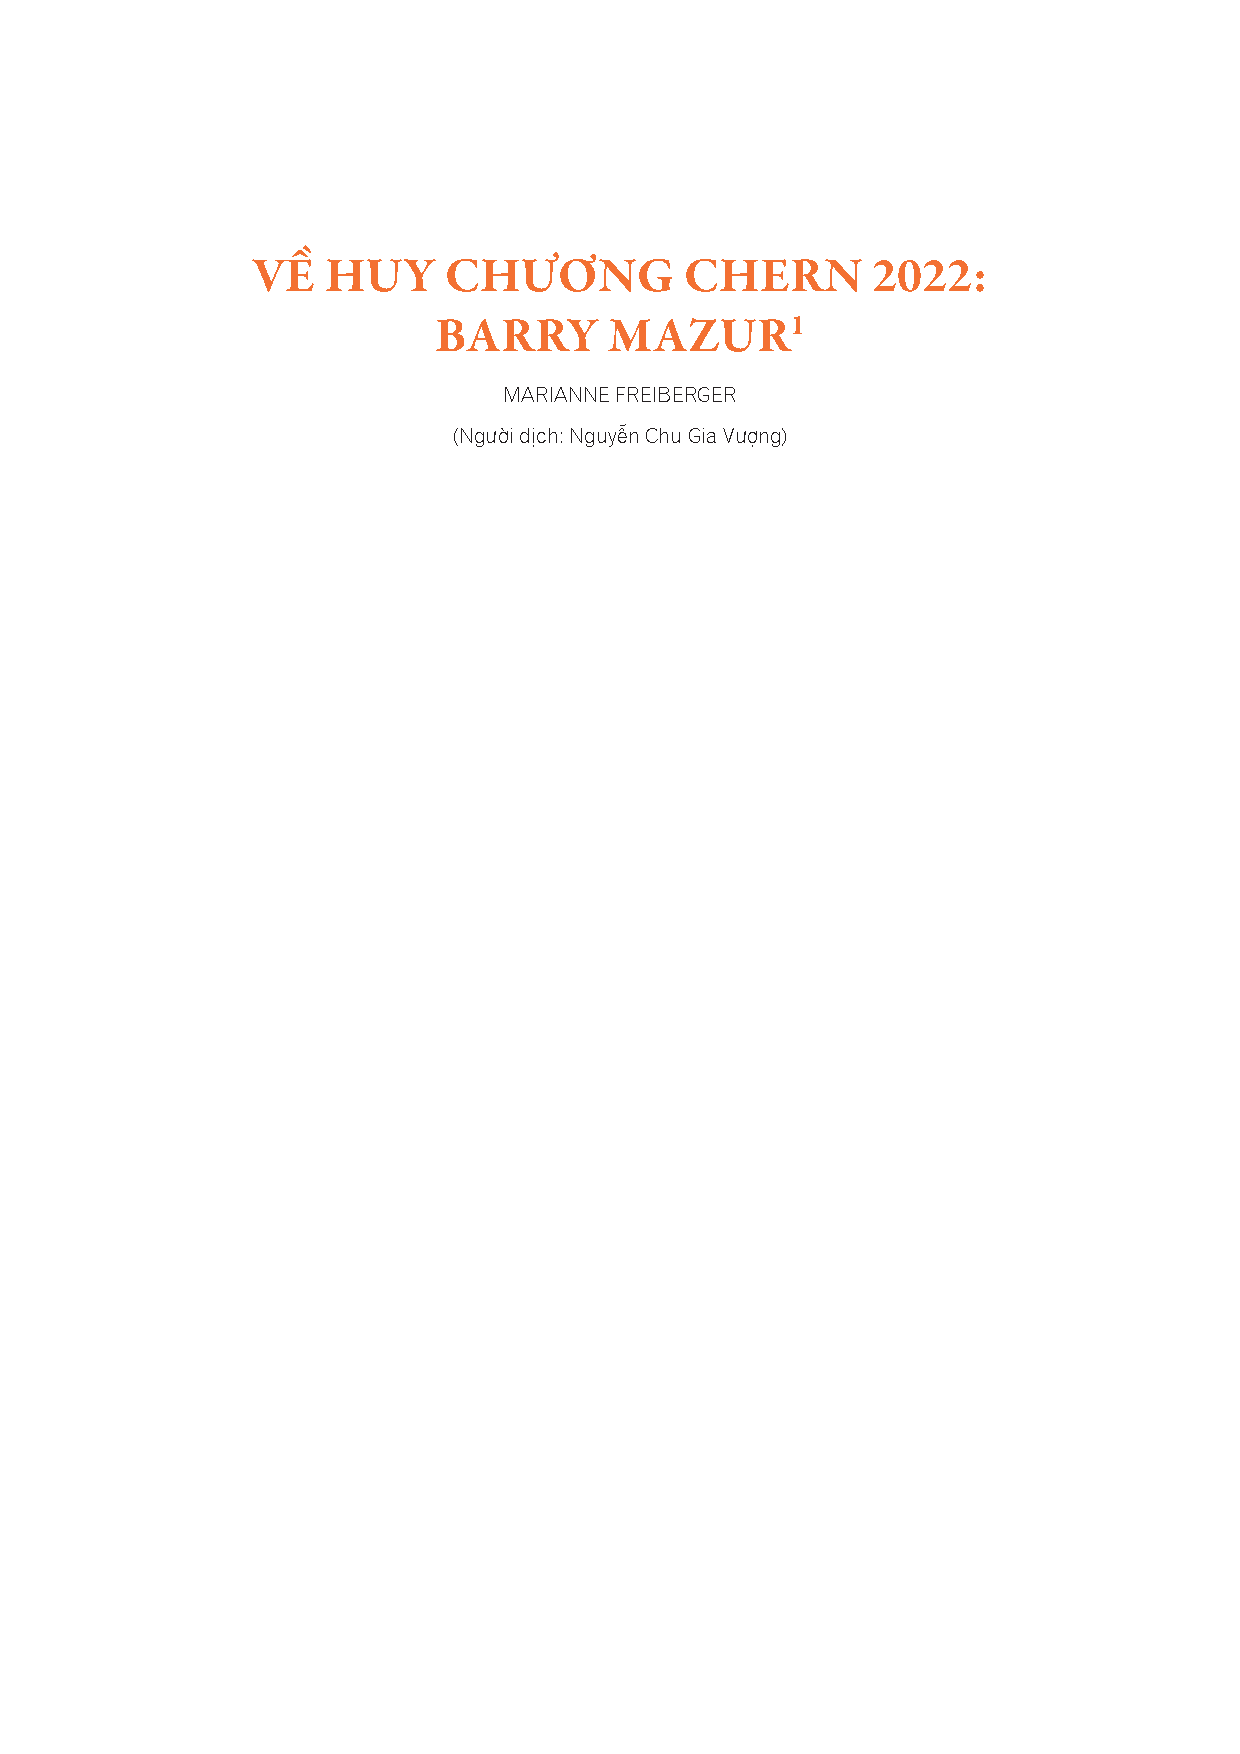
\includegraphics[scale=1]{../tieude.pdf}}}
\centering
\endgroup

\vspace*{150pt}

\tikzstyle{start} = [rectangle, rounded corners, minimum height=1cm,text centered, draw=black, fill=red!30]

\tikzstyle{end} = [rectangle, rounded corners, minimum height=1cm,text centered, draw=black, fill=blue!30]

\tikzstyle{mid} = [rectangle, rounded corners, minimum height=1cm,text centered, draw=black, fill=green!30]

\begin{multicols}{2}	
	$\pmb{1.}$ \textbf{\color{duongvaotoanhoc}Mở đầu}
	\vskip 0.1cm
	\textbf{\color{duongvaotoanhoc}Từ dải bện...}
	\vskip 0.1cm
	Dải bện đã tồn tại từ nhiều thế kỷ và được sử dụng khắp nơi vì mục đích trang trí cũng như trong đời sống, chẳng hạn trong sản xuất dây thừng hoặc dây cáp. Một dải bện có thể gồm ba sợi, hay cọng, được tết với nhau: cọng trái được vắt qua cọng giữa, rồi đến cọng phải, rồi lại cọng trái, rồi lại cọng phải, cứ thế lặp đi lặp lại (xem Hình $1$). Nhưng ``dải bện" cũng được dùng để chỉ mọi sự đan hay tết của nhiều cọng dây theo một cách nhất định. Trong Hình $2$ và Hình $3$ là một số thí dụ về các dải bện trang trí.
	\begin{figure}[H]
		\vspace*{-5pt}
		\centering
		\captionsetup{labelformat= empty, justification=centering}
		\includegraphics[width= 1\linewidth]{fig_01}
		\caption{\small\textit{\color{duongvaotoanhoc}Hình $1$. Dải bện cổ điển với ba cọng dây.}}
		\vspace*{-10pt}
	\end{figure}
	\begin{figure}[H]
		\vspace*{-5pt}
		\centering
		\captionsetup{labelformat= empty, justification=centering}
		\includegraphics[width= 1\linewidth]{fig_02}
		\caption{\small\textit{\color{duongvaotoanhoc}Hình $2$. Một dải bện trang trí.}}
		\vspace*{-10pt}
	\end{figure}
	\textbf{\color{duongvaotoanhoc}... đến lý thuyết bện}
	\vskip 0.1cm
	Các nhà toán học mô tả các dải bện bằng các mô hình trừu tượng, những đối tượng trung tâm của một lý thuyết toán học có tên ``lý thuyết bện". Lý thuyết này đóng một vai trò trung tâm trong toán học và len lỏi vào trong nhiều ngành toán học, cũng như các khoa học khác như vật lý, sinh học, tin học và mật mã.
	\begin{figure}[H]
		\vspace*{-5pt}
		\centering
		\captionsetup{labelformat= empty, justification=centering}
		\includegraphics[width= 1\linewidth]{fig_03a}
		\caption{\small\textit{\color{duongvaotoanhoc}Hình $3$. Một dải bện trang trí khác.}}
		\vspace*{-10pt}
	\end{figure}
	%	\vskip 0.1cm
	Bài viết này nhằm đem đến cho độc giả không làm toán một cái nhìn bao quát về lý thuyết bện. Chúng tôi sẽ đưa ra định nghĩa bện trong toán học, sau đó minh họa ứng dụng của chúng trong ba lĩnh vực: lý thuyết nút (toán học), lý thuyết thuật toán (toán học và tin học), và lý thuyết mật mã (toán học, tin học và viễn thông). Ngoài ra, chúng còn nhiều ứng dụng và tương tác qua lại khác với các phần khác của toán học, và với cả, chẳng hạn, vật lý thiên văn. Thực vậy, các đường từ trường trong khí quyển Mặt Trời tạo thành các dải bện mà độ phức tạp có liên hệ trực tiếp đến cường độ của từ trường.
	\vskip 0.1cm
	Lý thuyết bện là một lĩnh vực nghiên cứu rất tích cực ở Pháp, được tổ chức xung quanh nhóm nghiên cứu GDR TRESSES. Nhóm nghiên cứu này được thành lập năm $2000$ bởi Patrick Dehornoy với thời gian hoạt động $2$ năm, sau đó được gia hạn $4$ năm, từ $2003$ đến $2007$, dưới sự điều hành của Christian Blanchet (giáo sư tại Đại học Bretagne Sud), và từ năm $2008$ được điều hành bởi Luis Paris (giáo sư tại Đại học Bourgogne). Ngay từ đầu, một đặc thù quan trọng của nhóm nghiên cứu này là hòa trộn các nhà khoa học từ các lĩnh vực khác nhau. Nó gồm $18$ nhóm các nhà toán học và $2$ nhóm các nhà tin học, phân bố khắp nơi trên nước Pháp. Ngoài ra, những buổi họp mặt của nó còn có sự tham dự của nhiều nhà khoa học từ các nước khác. Uy tín quốc tế của GDR TRESSES đã được công nhận: tại hội nghị về lý thuyết bện ở Banff (Canada) vào tháng $4$ năm $2007$, GDR TRESSES được giới thiệu như một mô hình nghiên cứu kiểu mẫu.
	\begin{tBox}
		\begin{wrapfigure}{r}{0.4\linewidth}
			\vspace*{-15pt}
			\centering
			\captionsetup{labelformat= empty, justification=centering}
			\hspace*{-13pt}\includegraphics[width= 1.05\linewidth]{fig_Dehornoy}
			\hspace*{-13pt}\caption{\small\textit{\color{duongvaotoanhoc}Patrick Dehornoy.}}
			\vspace*{-10pt}
		\end{wrapfigure}
		Patrick Dehornoy ($1952-2019$) là nhà toán học Pháp được biết đến vì những công trình trong lý thuyết tập hợp và lý thuyết bện. Ông nguyên là giáo sư tại Đại học Caen và là thành viên kỳ cựu của Viện Đại học Pháp (Institut Universitaire de France). Ông là người sáng lập nhóm nghiên cứu GDR TRESSES, nơi tập trung các nghiên cứu về lý thuyết bện của nước Pháp.
	\end{tBox}
	\vskip 0.1cm
	$\pmb{2.}$ \textbf{\color{duongvaotoanhoc}Dải bện trong toán học}
	\vskip 0.1cm
	\textbf{\color{duongvaotoanhoc}Thế nào là một dải bện trong toán học?}
	\vskip 0.1cm
	\textit{Lý thuyết bện} tách khái niệm bện khỏi những dải bện mà ta vẫn thường nghĩ đến. Trước tiên, ta cố định một số tự nhiên $n$. Để tiện trình bày, ta sẽ lấy $n = 4$, mặc dù tất cả những gì được mô tả tiếp theo đây đúng với mọi giá trị của $n$. Chúng ta lấy hai tập hợp, mỗi tập hợp có $4$ vật (chẳng hạn những cái đinh) và để chúng trên bàn thành hai hàng dọc đối diện nhau (các chấm đen trong hình). Sử dụng bốn sợi dây, mà ta gọi là cọng, ta nối mỗi vật trong tập hợp thứ nhất với một vật trong tập hợp thứ hai. Một kết nối như vậy được gọi là một dải bện. Các cọng có thể vắt qua nhau, nhưng không được vòng ngược lại. Kết nối trong Hình $5$ không phải là một dải bện (theo nghĩa toán học).
	\begin{figure}[H]
		\vspace*{-10pt}
		\centering
		\captionsetup{labelformat= empty, justification=centering}
		\includegraphics[width= 0.465\linewidth]{fig_04}\quad
		\includegraphics[width= 0.465\linewidth]{fig_05}
		\caption{\small\textit{\color{duongvaotoanhoc}Hình $4$. Một dải bện \hspace*{18pt} Hình $5$. Đây không \hspace*{10pt}\\
				\hspace*{20pt}toán học.\hspace*{45pt} phải một dải bện. }}
		\vspace*{-10pt}
	\end{figure}	
	Trong Hình $6$ là hai dải bện khác nhau. Trong khi đó, hai dải bện trong Hình $7$ là giống nhau, vì chúng có thể nhận được từ nhau bằng cách ``xê dịch" các cọng.
	\begin{figure}[H]
		\vspace*{-5pt}
		\centering
		\captionsetup{labelformat= empty, justification=centering}
		\includegraphics[width= 1\linewidth]{fig_06}
		\caption{\small\textit{\color{duongvaotoanhoc}Hình $6$. Hai dải bện khác nhau.}}
		\vspace*{-5pt}
	\end{figure}
	\begin{figure}[H]
		\vspace*{2pt}
		\centering
		\captionsetup{labelformat= empty, justification=centering}
		\includegraphics[width= 0.97\linewidth]{fig_07}
		\caption{\small\textit{\color{duongvaotoanhoc}Hình $7$. Hai dải bện giống nhau.}}
		\vspace*{-10pt}
	\end{figure}
	Một dải bện cũng có thể được coi như một chuỗi các đường đi của $4$ hạt không gặp nhau. Ở đây, tập hợp các điểm xuất phát trùng với tập hợp các điểm đến. Thí dụ, các quỹ đạo của $4$ hạt được thể hiện ở nửa trên của Hình $8$ tương ứng với dải bện ở nửa dưới. Một cách nôm na, các dải bện có thể được xem như những điệu nhảy mà ở đó, mỗi vũ công kết thúc ở vị trí của một vũ công khác.
	\begin{figure}[H]
		\vspace*{-5pt}
		\centering
		\captionsetup{labelformat= empty, justification=centering}
		\includegraphics[width= 0.475\linewidth]{fig_08}
		\caption{\small\textit{\color{duongvaotoanhoc}Hình $8$. Hai cách nhìn của cùng một dải bện.}}
		\vspace*{-10pt}
	\end{figure}
	\textbf{\color{duongvaotoanhoc}Ghép các dải bện}
	\vskip 0.05cm
	Từ hai dải bện $\alpha$ và $\beta$, ta có thể xây dựng một phép thứ ba, ký hiệu là $\alpha \beta$ và được gọi là dải bện hợp thành của $\alpha$ và $\beta$, bằng cách ghép chúng với nhau. Trong Hình $9$ là hai dải bện (bên trên) và hợp thành của chúng (bên dưới).
	\begin{figure}[H]
		\vspace*{-5pt}
		\centering
		\captionsetup{labelformat= empty, justification=centering}
		\includegraphics[width= 0.97\linewidth]{fig_09}
		\caption{\small\textit{\color{duongvaotoanhoc}Hình $9$. Hợp thành của hai dải bện.}}
		\vspace*{-5pt}
	\end{figure}
	Một thí dụ khác về phép hợp thành được minh họa trong Hình $10$.
	\begin{figure}[H]
		\vspace*{-5pt}
		\centering
		\captionsetup{labelformat= empty, justification=centering}
		\includegraphics[width= 0.97\linewidth]{fig_10}
		\caption{\small\textit{\color{duongvaotoanhoc}Hình $10$. Hợp thành của hai dải bện khác.}}
		\vspace*{-10pt}
	\end{figure}
	Bạn đọc có kinh nghiệm hẳn đã để ý rằng dải bện $\alpha \beta$ có thể khác với dải bện $\beta \alpha$: điều này xảy ra với thí dụ trong Hình $9$, nhưng không đúng với thí dụ trong Hình $10$.
	\vskip 0.1cm
	Dải bện trong Hình $11$ được gọi là \textit{dải bện tầm thường}. Dễ thấy hợp của một dải bện $\alpha$ bất kỳ với dải bện tầm thường, từ bên trái hay từ bên phải, vẫn là $\alpha$.
	\begin{figure}[H]
		\vspace*{-5pt}
		\centering
		\captionsetup{labelformat= empty, justification=centering}
		\includegraphics[width= 0.47\linewidth]{fig_11}
		\caption{\small\textit{\color{duongvaotoanhoc}Hình $11$. Dải bện tầm thường.}}
		\vspace*{-10pt}
	\end{figure}
	Nếu ta đặt một tấm gương vuông góc với mặt bàn ở cạnh hàng đinh thứ hai, ảnh phản chiếu trong gương của dải bện $\alpha$ được gọi là dải bện đối xứng của $\alpha$ (xem Hình $12$). Hợp thành của một dải bện với dải bện đối xứng của nó là dải bện tầm thường. Bạn đọc có thể dễ dàng kiểm chứng với thí dụ trong Hình $12$.
	\begin{figure}[H]
		\vspace*{-5pt}
		\centering
		\captionsetup{labelformat= empty, justification=centering}
		\includegraphics[width= 0.97\linewidth]{fig_12}
		\caption{\small\textit{\color{duongvaotoanhoc}Hình $12$. Một dải bện và dải bện đối xứng của~nó.}}
		\vspace*{-5pt}
	\end{figure}
	\textbf{\color{duongvaotoanhoc}Từ dải bện đến nhóm bện}
	\vskip 0.1cm
	Những dải bện, như chúng ta vừa định nghĩa, cùng với phép hợp thành tạo thành cái mà các nhà toán học gọi là \textit{nhóm bện}. Chúng ta có một nhóm bện [gồm các dải bện có] hai cọng, một nhóm bện ba cọng, v.v. Nhóm bện một cọng chỉ gồm dải bện tầm thường, vì một cọng thì không thể được bện, dù nó có thể được buộc thắt nút (xem Hình $13$).
	\begin{figure}[H]
		\vspace*{-5pt}
		\centering
		\captionsetup{labelformat= empty, justification=centering}
		\includegraphics[width= 0.45\linewidth]{fig_13}
		\caption{\small\textit{\color{duongvaotoanhoc}Hình $13$. Cọng buộc thắt nút.}}
		\vspace*{-10pt}
	\end{figure}
	Phép hợp thành của các dải bện tuân theo một số quy tắc mà đối với các nhà toán học cũng quan trọng không kém, nếu không nói là hơn, chính các dải bện.
	Nguồn gốc của lý thuyết bện
	\vskip 0.1cm
	Nghiên cứu toán học về các dải bện thường được cho là bắt đầu từ bài báo năm $1925$ của Emil Artin [$4$], trong đó ông mô tả khái niệm dải bện dưới nhiều khía cạnh khác nhau, cái thì hiển nhiên như ``một chuỗi các cọng dây được kéo căng và quấn vào nhau", những cái khác toán học hơn, chẳng hạn như nhóm được cho bởi ``các phần tử sinh và các quan hệ", hay như ``nhóm các tự đẳng cấu của một nhóm tự do", hay như  ``nhóm các phép đẳng luân của một đĩa bị thủng". Chính sự đa dạng của các cách tiếp cận khác nhau này tạo nên tính hấp dẫn của các nhóm bện.
	\begin{tBox}
		\begin{wrapfigure}{l}{0.4\linewidth}
			\vspace*{-15pt}
			\centering
			\captionsetup{labelformat= empty, justification=centering}
			\includegraphics[width= 1.1\linewidth]{fig_Artin}
			\caption{\small\textit{\color{duongvaotoanhoc}Emil Artin}}
			\vspace*{-15pt}
		\end{wrapfigure}
		Emil Artin ($1898-1962$) là nhà toán học người Áo. Ông làm việc ở Đức (chủ yếu ở Hamburg) đến năm $1937$. Ông sang Mỹ và làm giáo sư tại Đại học Indiana từ năm $1938$ đến năm $1946$, rồi tại Đại học Princeton từ năm $1946$ đến năm $1958$. Ông là một trong những nhà đại số xuất sắc nhất thế kỷ $20$. Đặc biệt, ông là người khai sinh lý thuyết bện.
	\end{tBox}
	$\pmb{3.}$ \textbf{\color{duongvaotoanhoc}Từ dải bện đến lý thuyết nút}
	\vskip 0.1cm
	\textbf{\color{duongvaotoanhoc}Nút trong toán học là gì?}
	\vskip 0.1cm
	Một \textit{nút} trong toán học là một vòng dây khép kín (không có hai đầu, xem Hình $14$). Một \textit{cuộn dây gồm hai thành phần} được tạo bởi hai vòng dây khép kín (xem Hình $15$), một \textit{cuộn dây gồm ba thành phần} được tạo bởi ba vòng dây khép kín, v.v. \textit{Lý thuyết nút} là nhánh của tô--pô nghiên cứu các nút và các cuộn. Trong tô--pô, hình cầu không phân biệt với hình lập phương, còn cái bánh vòng và tách trà là một. Người ta không xét đến các thuộc tính như độ dài hay góc, mục đích là hiểu các tính chất bất biến đối với sự xoắn, kéo dãn hay nén.
	\begin{figure}[H]
		\vspace*{-10pt}
		\centering
		\captionsetup{labelformat= empty, justification=centering}
		\includegraphics[height= 0.4\linewidth]{fig_14}\quad
		\includegraphics[height= 0.4\linewidth]{fig_15}
		\caption{\small\textit{\color{duongvaotoanhoc}Hình $14$. Một nút. Hình $15$. Một cuộn dây gồm hai thành phần.}}
		\vspace*{-10pt}
	\end{figure}
	Ngoài toán học, đặc biệt là tô--pô, lý thuyết nút có những ứng dụng trong các bài toán sinh học và hóa học. Chẳng hạn, nó được dùng trong nghiên cứu các phân tử đồng phân (có cùng công thức hóa học nhưng được sắp xếp khác nhau) hoặc trong nghiên cứu về tác động của một số enzyme đối với ADN.
	\vskip 0.1cm
	\textbf{\color{duongvaotoanhoc}Nguồn gốc của lý thuyết nút}
	\vskip 0.1cm
	Đóng góp đáng kể đầu tiên vào lý thuyết nút có lẽ là của Sir William Thomson (tức Kelvin) với thuyết ``xoáy nguyên tử" của ông. Năm $1867$, sau khi quan sát các vòng khói được tạo ra từ thí nghiệm của Peter Tait, nhà vật lý người Scotland, Thomson kết luận rằng các nguyên tử là những nút của ``những cuộn xoáy trong ê--te truyền ánh sáng". Theo đó, các nguyên tố hóa học ứng với các nút hoặc cuộn dây. Từ ý tưởng này, Peter Tait bắt đầu phân loại các nút, với niềm tin rằng ông đang tạo ra một bảng nguyên tố hóa học.
	\begin{tBox}
		\begin{wrapfigure}{l}{0.4\linewidth}
			\vspace*{-15pt}
			\centering
			\captionsetup{labelformat= empty, justification=centering}
			\includegraphics[width= 1.1\linewidth]{fig_William}
			\caption{\small\textit{\color{duongvaotoanhoc}William~Thomson.}}
			\vspace*{-10pt}
		\end{wrapfigure}
		Sir William Thomson ($1824-1907$) là nhà vật lý học, nhà toán học và kỹ sư người Scotland. Ông được coi là một trong những nhà vật lý học hàng đầu của thế kỷ~$19$.
	\end{tBox}
	\textbf{\color{duongvaotoanhoc}Bài toán phân biệt hai nút}
	\vskip 0.1cm
	Bài toán trung tâm của lý thuyết nút là phân biệt, và xa hơn là phân loại, các nút. Phân biệt có nghĩa là quyết định xem liệu hai hình vẽ nút (hoặc cuộn dây) có biểu diễn cùng một nút (hoặc cuộn dây) hay không. Trong những năm $1920$, hai nhà toán học Mỹ Alexander và Briggs [$2$] và nhà toán học Đức Reidemeister [$16$], độc lập với nhau, đề xuất một thuật toán giải quyết một phần bài toán này. Thuật toán này có thể trả lời khẳng định nếu hai hình vẽ biểu diễn cùng một nút (hoặc cuộn), nhưng nó không trả lời trong trường hợp ngược lại. Nói cách khác, ta có thể nói hai nút giống nhau hay không, nhưng không thể nói hai nút có khác nhau hay không. Độc giả có thể cảm thấy điều này thật vô lý, nhưng nó là một nghịch lý thường thấy trong toán học. Hãy tưởng tượng bạn đang chờ ai đó. Bạn tự nhủ: ``Nếu cậu ấy đến, đó đúng là một người bạn." Nhưng nếu người đó không đến, bạn sẽ không biết đó có phải một người bạn hay không.
	\vskip 0.05cm
	Để phân biệt các nút, người ta sử dụng những cái mà các nhà toán học gọi là những \textit{bất biến}. Người ta gán cho mỗi hình vẽ cái nút một đối tượng (thường là một số hoặc một đa thức) chỉ phụ thuộc vào cái nút mà không phụ thuộc vào cách nó được vẽ. Nếu hai nút có những bất biến khác nhau thì chúng là hai nút khác nhau. Nếu không, ta chưa thể kết luận được gì.
	\vskip 0.1cm
	\textbf{\color{duongvaotoanhoc}Từ dải bện đến nút}
	\begin{figure}[H]
		\vspace*{-10pt}
		\centering
		\captionsetup{labelformat= empty, justification=centering}
		\includegraphics[width= 1\linewidth]{fig_16}
		\caption{\small\textit{\color{duongvaotoanhoc}Hình $16$. Dải bện đóng.}}
		\vspace*{-10pt}
	\end{figure}
	Từ một dải bện, ta có thể tạo ra một cuộn dây (hoặc một nút) bằng cách nối các đầu của dải bện với nhau, như minh họa trong Hình $16$. Một cuộn dây như vậy được gọi là một dải bện đóng. Alexander [$1$] đã chứng minh rằng mọi cuộn dây đều có thể được tạo ra theo cách này. Bạn đọc có thể thử với các thí dụ trong Hình $14$ và Hình $15$. Sau đó, Markov [$15$] đưa ra một thuật toán không hoàn toàn để xác định liệu hai dải bện cho trước có tạo thành cùng một cuộn dây (nhưng nó có thể không trả lời). Đây là hai kết quả cốt yếu để áp dụng lý thuyết bện vào các nút. Đặc biệt, chúng là điểm bắt đầu của sự đổi mới sâu sắc trong lý thuyết nút trong thập niên $1980$,
	với những công trình của Jones [$12$, $13$] và những bất biến được định nghĩa từ lý thuyết bện.
	\vskip 0.01cm
	\begin{tBox}
		\begin{wrapfigure}{l}{0.45\linewidth}
			\vspace*{-15pt}
			\centering
			\captionsetup{labelformat= empty, justification=centering}
			\hspace*{2pt}\includegraphics[width= 1.1\linewidth]{fig_Alexander}
			\caption{\small\textit{\color{duongvaotoanhoc}Alexander.}}
			\vspace*{-10pt}
		\end{wrapfigure}
		James W. Alexander ($1888-1971$) là một nhà toán học nổi tiếng người Mỹ. Là một trong những thành viên đầu tiên của Viện Nghiên cứu Cao cấp Princeton (từ $1933$ đến $1951$), ông đồng thời là giáo sư tại Đại học Princeton (từ $1920$ đến $1951$). Ông là một trong những người tiên phong của tô--pô đại số và lý thuyết nút. Ông cũng là một nhà leo núi cừ khôi, từng chinh phục được nhiều đỉnh cao. Về cuối đời, ông trở nên đơn độc và ẩn dật. Ông được biết đến như một người theo chủ nghĩa xã hội tích cực và danh tiếng của ông khiến ông bị chủ nghĩa MacCarthy để ý. Ông không xuất hiện trước công chúng kể từ năm $1954$, sau khi ký tên vào một bức thư ủng hộ Robert Oppenheimer.
	\end{tBox}
	
	\vspace*{-8pt}
	\begin{tBox}
		\begin{wrapfigure}{r}{0.4\linewidth}
			\vspace*{-15pt}
			\centering
			\captionsetup{labelformat= empty, justification=centering}
			\hspace*{-10pt}\includegraphics[width= 1.1\linewidth]{fig_Jones}
			\caption{\small\textit{\color{duongvaotoanhoc}Jones.}}
			\vspace*{-15pt}
		\end{wrapfigure}
		Vaughan F.R. Jones ($1952-2020$) là nhà toán học người New Zealand nổi tiếng với những công trình về các đại số von Neumann, các bất biến nút và lý thuyết trường bảo giác. Ông được trao Huy chương Fields năm $1990$ và là giáo sư ($1985-2011$) rồi giáo sư danh dự ($2011$ đến khi mất) tại Đại học California tại Berkeley. Các công trình của ông về bất biến nút dẫn tới những lời giải bất ngờ cho nhiều bài toán cổ điển trong lý thuyết nút và tô--pô thấp chiều.
	\end{tBox}
	\vskip 0.05cm
	\textbf{\color{duongvaotoanhoc}Phân biệt hai dải bện}
	\vskip 0.1cm
	Khác với nút, với dải bện tồn tại các thuật toán để xác định xem hai dải bện có giống nhau hay không. Nhiều thuật toán trong số này rất nhanh và đã được đưa vào các phần mềm tính toán như GAP hay MAGMA. Sự tồn tại của các thuật toán này liên quan đến việc các dải bện không chỉ là những đối tượng tô--pô, mà còn là những \textit{đối tượng đại số}, bởi như đã thấy, ta có thể áp dụng phép hợp thành lên chúng. Dưới đây là một cách xác định liệu hai dải bện có bằng nhau hay không. Rất có thể quá trình này đã được Artin biết đến từ năm $1925$.
	\vskip 0.1cm
	Xét hai (hình) dải bện $\alpha$ và $\beta$.
	\vskip 0.1cm
	Bước $1$: Gọi $\tilde \beta$ là dải bện đối xứng của $\beta$. Để ý rằng $\alpha$ và $\beta$ là cùng một dải bện nếu và chỉ nếu dải bện hợp thành $\alpha \tilde \beta$ là tầm thường. Đặt $\gamma = \alpha \tilde \beta$. Bài toán trở thành xác định xem $\gamma$ có phải dải bện tầm thường hay không.
	\vskip 0.1cm
	Bước $2$: Để $\gamma$ là dải bện tầm thường thì cọng đi từ đinh trên cùng bên trái phải nối đến đinh trên cùng bên phải, cọng từ đinh thứ hai bên trái nối đến đinh thứ hai bên phải, v.v. Ta kiểm tra điều này với $\gamma$. Nếu $\gamma$ không thỏa mãn thì nó không tầm thường. Thí dụ, dải bện trong Hình $17$ không tầm thường vì cọng đi từ đinh dưới cùng bên trái nối đến đinh thứ hai từ trên xuống ở bên phải. Còn nếu $\gamma$ thỏa mãn, ta chuyển sang bước $3$.
	\begin{figure}[H]
		\vspace*{-5pt}
		\centering
		\captionsetup{labelformat= empty, justification=centering}
		\includegraphics[width= 0.48\linewidth]{fig_17}
		\caption{\small\textit{\color{duongvaotoanhoc}Hình $17$. Một dải bện không tầm thường.}}
		\vspace*{-10pt}
	\end{figure}
	Bước $3$: Nếu bỏ đi cọng dây trên cùng, ta nhận được một dải bện $\gamma'$ gồm $3$ cọng (có thể làm điều này vì cọng dây nối đinh trên cùng bên trái với đinh trên cùng bên phải). Giả sử ta đã biết cách phân biệt hai dải bện gồm $3$ cọng. Để $\gamma$ là tầm thường thì $\gamma'$ cũng phải tầm thường. Thí dụ, dải bện $\gamma$ trong Hình $18$ không tầm thường vì $\gamma'$ không tầm thường. Nếu $\gamma'$ là tầm thường, ta chuyển sang bước~$4$.
	\begin{figure}[H]
		\vspace*{-5pt}
		\centering
		\captionsetup{labelformat= empty, justification=centering}
		\includegraphics[width= 0.48\linewidth]{fig_18}
		\caption{\small\textit{\color{duongvaotoanhoc}Hình $18$. Xóa một cọng dây.}}
		\vspace*{-10pt}
	\end{figure}
	Bước $4$: Tới bước này, ba cọng bên dưới của dải bện của chúng ta là các đoạn thẳng, trong khi cọng bị xóa vắt qua chúng, như minh họa trong Hình $19$. Tới đây cần những công cụ toán học phức tạp hơn, nhưng bạn đọc có thể nắm được rằng người ta biết cách xử lý trường hợp này một cách không quá khó khăn, nhưng cần những công cụ mà trong khuôn khổ bài viết này không đủ chỗ để giải thích.
	\begin{figure}[H]
		\vspace*{-5pt}
		\centering
		\captionsetup{labelformat= empty, justification=centering}
		\includegraphics[width= 0.48\linewidth]{fig_19}
		\caption{\small\textit{\color{duongvaotoanhoc}Hình $19$. Một cọng vắt qua các cọng khác.}}
		\vspace*{-10pt}
	\end{figure}
	$\pmb{4.}$ \textbf{\color{duongvaotoanhoc}Từ dải bện đến thuật toán}
	\vskip 0.1cm
	\textbf{\color{duongvaotoanhoc}Thuật toán và ngôn ngữ}
	\vskip 0.1cm
	Nếu bạn chỉ đường cho một người khách đến chơi nhà mình, bạn đang tạo ra (và cho thực hiện) một thuật toán đấy! Một \textit{thuật toán} là một dãy các chỉ dẫn (toán học hoặc không) được định nghĩa rõ ràng nhằm thực hiện một công việc nào đó. Nếu thuật toán đúng, kết quả nhận được sẽ là kết quả mong muốn và vị khách sẽ tìm được đường đến đúng nhà bạn. Nếu thuật toán sai, kết quả có thể ngoài dự kiến. Trong tin học, thuật toán cho phương pháp, và việc lập trình chuyển nó thành dạng các câu lệnh cho máy tính.
	\vskip 0.1cm
	Một khái niệm quan trọng trong khoa học thuật toán là từ và ngôn ngữ. Với một nhà nghiên cứu thuật toán, một \textit{bảng chữ cái} là một tập hợp hữu hạn mà các phần tử được gọi là các chữ cái, một từ là một dãy hữu hạn các chữ cái, và một \textit{ngôn ngữ} là một tập hợp các từ. Thí dụ, tập hợp $\mathcal A = \{a, b\}$ là một bảng chữ cái, các dãy $b, ab, aab, aaab$ là các từ, và tập hợp $\{b, ab, aab, aaab, aaaab, \dots\}$ là một ngôn ngữ. Một thí dụ khác: ADN là thuật toán nền tảng để xây dựng nên sự sống. Mỗi phân tử ADN là một chuỗi được tạo thành từ bốn phần tử: adenine (A), thymine (T), cytosine (C) và guanine (G). Số phần tử cũng như thứ tự sắp xếp của chúng sẽ quyết định tạo ra con muỗi hay con sư tử. Một cách ngắn gọn: mỗi từ tạo thành từ bảng chữ cái $\{A, T, C, G\}$ biểu diễn một thuật toán để tạo ra một sinh vật, và tập hợp tất cả các sinh vật có thể được xem như một ngôn ngữ trên bảng chữ cái $\{A, T, C, G\}$. Đó là khởi đầu việc mô hình hóa trong di truyền học.
	\vskip 0.1cm
	\textbf{\color{duongvaotoanhoc}Từ dải bện đến các từ}
	\vskip 0.1cm
	Chúng ta có thể biểu diễn các dải bện bằng các từ mà không cần đến hình vẽ. Bảng chữ cái được dùng ở đây là $\mathcal A = \{a, b, c, A, B, C\}$. Mỗi chữ cái trong bảng chữ cái này tương ứng với một dải bện ``sơ cấp", xem Hình $20$. Cho một dải bện $\alpha$ bất kỳ, bằng cách cắt $\alpha$ thành các lát nhỏ theo chiều dọc, ta có thể dễ dàng nhận thấy rằng $\alpha$ là hợp thành của nhiều dải bện sơ cấp. Nói cách khác, $\alpha$ có thể được viết như một từ trên bảng chữ cái $\mathcal A$. Thí dụ, dải bện trong Hình $21$ tương ứng với từ $aabC$.
	\begin{figure}[H]
		\vspace*{-5pt}
		\centering
		\captionsetup{labelformat= empty, justification=centering}
		\includegraphics[width= 0.65\linewidth]{fig_20}
		\caption{\small\textit{\color{duongvaotoanhoc}Hình $20$. Dải bện sơ cấp.}}
		%		\vspace*{-5pt}
	\end{figure}
	\begin{figure}[H]
		\vspace*{5pt}
		\centering
		\captionsetup{labelformat= empty, justification=centering}
		\includegraphics[width= 0.48\linewidth]{fig_21}
		\caption{\small\textit{\color{duongvaotoanhoc}Hình $21$. Dải bện $aabC$.}}
		\vspace*{-10pt}
	\end{figure}
	Nhóm bện được đặc trưng bởi hai tính chất sau:
	\vskip 0.1cm
	$1$. Mọi dải bện đều viết được dưới dạng một từ trên bảng chữ cái $\mathcal A = \{a, b, c, A, B, C\}$;
	\vskip 0.1cm
	$2$. Ta có các đẳng thức sau:
	\begin{align*}
		&aA = Aa = \varepsilon\,, bB = Bb = \varepsilon\,, cC = Cc = \varepsilon\,\\
		&aba = bab\,, ac = ca\,, bcb = cbc\,,
	\end{align*}
	ở đó $\varepsilon$ chỉ từ rỗng, tức là từ có độ dài $0$, không có chữ cái nào. Đẳng thức $aba = bab$ được minh họa trong Hình $22$.
	\begin{figure}[H]
		\vspace*{-5pt}
		\centering
		\captionsetup{labelformat= empty, justification=centering}
		\includegraphics[width= 1\linewidth]{fig_22}
		\caption{\small\textit{\color{duongvaotoanhoc}Hình $22$. Đẳng thức $aba = bab$.}}
		\vspace*{-10pt}
	\end{figure}
	\textbf{\color{duongvaotoanhoc}Bài toán từ và bài toán liên hợp}
	\vskip 0.1cm
	Tồn tại một thuật toán nhận đầu vào là hai từ trên bảng chữ cái $\mathcal A = \{a, b, c, A, B, C\}$ và quyết định liệu chúng có biểu diễn cùng một dải bện hay không. Một thuật toán như vậy được gọi là một lời giải cho \textit{bài toán từ}. Bạn đọc có lẽ cũng đã để ý rằng bài toán này rõ ràng chính là một bài toán đã được nói đến ở bên trên: xác định xem hai hình vẽ có biểu diễn cùng một dải bện hay không.
	\vskip 0.1cm
	Và đây là một bài toán nữa về dải bện mà chúng ta có thuật toán để giải. Cho hai dải bện $\alpha$ và $\beta$, chúng ta có thể trả lời rằng có hay không một dải bện $\gamma$ sao cho $\alpha \gamma = \gamma \beta$, và trong trường hợp câu trả lời là khẳng định, ta còn biết cách tìm tất cả các $\gamma$ thỏa mãn. Độc giả có thể nhận ra rằng bài toán này chính là giải phương trình $\alpha X = X \beta$. Nhắc lại rằng giải phương trình $\alpha X = X \beta$ nghĩa là tìm tập hợp tất cả các $X$ thỏa mãn đẳng thức này. Nếu không tồn tại $X$ như vậy, tập hợp này là rỗng. Một thuật toán giải phương trình $\alpha X = X \beta$ với $\alpha$ và $\beta$ cho trước được gọi là một lời giải cho \textit{bài toán liên hợp}.
	\vskip 0.1cm
	\textbf{\color{duongvaotoanhoc}Bài toán quyết định}
	\vskip 0.1cm
	Bài toán từ và bài toán liên hợp thuộc vào họ các bài toán trong toán học, rất gần với thuật toán và tin học, được gọi là ``các bài toán quyết định". Các bài toán quyết định nhận được sự quan tâm ngày càng tăng không chỉ vì ứng dụng của chúng trong nhiều lĩnh vực khác, mà còn vì chính những thay đổi của khái niệm chứng minh toán học. Quả vậy, ngày nay người ta phân biệt khái niệm chứng minh và khái niệm chứng minh ``thực sự", tức là phải xây dựng được lời giải. Một xây dựng như vậy được thực hiện bởi một thuật toán và độ phức tạp (tức thời gian tính toán) của nó là một dữ liệu cần được tính toán và được quan tâm bởi những kỹ sư tin học muốn sử dụng nó.
	\vskip 0.1cm
	\textbf{\color{duongvaotoanhoc}Kết quả toán học không xây dựng bằng thuật toán}
	\vskip 0.1cm
	Định lý sau đây là một thí dụ về một chứng minh không xây dựng. Nó thường được biết đến dưới cái tên \textit{định lý bánh mỳ kẹp} (xem Hình $23$).
	\begin{figure}[H]
		\vspace*{-5pt}
		\centering
		\captionsetup{labelformat= empty, justification=centering}
		\includegraphics[width= 0.9\linewidth]{fig_23}
		\caption{\small\textit{\color{duongvaotoanhoc}Hình $23$. Định lý bánh mỳ kẹp không áp dụng được trong thực tế.}}
		\vspace*{-5pt}
	\end{figure}
	\textbf{\color{duongvaotoanhoc}Định lý:} Với mọi cái bánh mỳ kẹp gồm bánh mỳ, giăm--bông và phô--mai, luôn tồn tại một nhát cắt đều, tức là sao cho hai phần nhận được có lượng bánh mỳ, giăm bông và phô--mai bằng nhau.
	\vskip 0.1cm
	Dù biết là một nhát cắt như thế tồn tại, ta không biết cách nào tìm ra nó. Tuy nhiên, không như vẻ bề ngoài của nó, lý thuyết dẫn đến định lý này không hề vô dụng một chút nào (hình ảnh bánh mỳ kẹp chỉ là minh họa dễ hiểu). Chẳng hạn, với chính những kỹ thuật đó, các nhà toán học đã thiết lập được sự tồn tại của những enzyme có tên topoisomerase có khả năng làm biến đổi hình dạng của ADN.
	\vskip 0.1cm
	\textbf{\color{duongvaotoanhoc}Các bài toán quyết định về dải bện}
	\vskip 0.1cm
	Thuật toán trong các nhóm bện được nghiên cứu đặc biệt tích cực. Nhiều bài toán quyết định như bài toán từ hay bài toán liên hợp, được Garside [$11$] giải quyết vào năm $1969$. Không có thêm nhiều đột phá, cho đến khi cuốn sách của Epstein et al. được xuất bản. Cuốn sách này mô tả nhiều thuật toán bắt nguồn từ lý thuyết ô--tô--mát để giải các bài toán quyết định trong nhóm bện.
	\vskip 0.1cm
	Frank A. Garside đang là giám đốc một trường nam sinh khi ông bắt đầu làm nghiên cứu sinh tiến sỹ tại Oxford vào năm $1968$. Với một công việc toàn thời gian, ông biết rằng tốc độ làm việc của mình sẽ chậm và lựa chọn một chủ đề xa với những xu hướng chủ đạo đương thời: ông tìm cách giải bài toán liên hợp trong nhóm bện. Ông phát hiện ra một cấu trúc khi đó còn chưa được biết đến nhưng đến nay đã có vô số ứng dụng và dạng tổng quát hóa vượt xa chủ đề luận án của ông. Mặc dù đóng góp của ông khởi nguồn cho một lĩnh vực nghiên cứu vẫn còn rất tích cực đến tận ngày nay, trong suốt đời ông chỉ công bố đúng một bài báo.
	\vskip 0.1cm
	Dehornoy và tác giả bài viết này [$9$] đưa ra một bộ khung rõ ràng và tổng quát hơn để nghiên cứu các bài toán quyết định trong nhóm bện: nhóm Garside. Ý tưởng ban đầu là tách riêng một số tính chất tổ hợp của các nhóm bện: đại loại nghĩa là tạo ra một mô hình ít ràng buộc hơn và chỉ sử dụng những công cụ từ lý thuyết ngôn ngữ và tổ hợp, những lĩnh vực đặc biệt thích hợp để xử lý những vấn đề thuật toán. Dưới sự thúc đẩy của các trường phái Pháp, Mỹ, Hàn Quốc và Israel, nhiều bước tiến lớn đã được đạt tới, giúp hiểu rõ các cấu trúc này. Nhiều ứng dụng đã xuất hiện, đặc biệt là trong mật mã.
	\vskip 0.1cm
	$\pmb{5.}$ \textbf{\color{duongvaotoanhoc}Từ dải bện đến mật mã}
	\vskip 0.1cm
	\textbf{\color{duongvaotoanhoc}Mật mã}
	\vskip 0.1cm
	Mật mã là ngành nghiên cứu những cách gửi các thông điệp bí mật trên các kênh liên lạc công khai. Nó được coi như một nhánh của cả toán học, tin học lẫn khoa học truyền thông, và có rất nhiều ứng dụng, chẳng hạn như trong thẻ ngân hàng, trong thương mại điện tử hay trong bảo mật của điện thoại di động.
	\begin{figure}[H]
		\vspace*{-5pt}
		\centering
		\captionsetup{labelformat= empty, justification=centering}
		\begin{tikzpicture}[scale=0.6, node font=\scriptsize]
			\node (a) [start]{Anh yêu em};
			\node (b) [end, xshift = 3cm]{Máy mã hóa};
			\node [yshift = 1cm,xshift = 3cm]{Bob};
			\node [mid, yshift = -2cm,xshift = 3cm]{AC$2$KJL\%PBGH$7$IRVF};
			\node (c) [xshift = 5.5cm]{\includegraphics[scale=0.8]{keya.JPG}};
			\node [xshift = 5.1cm, yshift = -0.7cm]{Chìa khóa của Bob};
			\draw[-stealth] (a) -- (b);
			\draw[-stealth] (c) -- (b);
			\draw[dashed] (-1.2,-1.6) -- (10,-1.6);
			\draw[dashed] (-1.2,-4.9) -- (10,-4.9);
			\node (d) [start, yshift = -4cm]{Anh yêu em};
			\node (e) [end, xshift = 3cm, yshift = -4cm]{Máy giải mã};
			\node (g) [mid, yshift = -2cm,xshift = 3cm]{AC$2$KJL\%PBGH$7$IRVF};
			\node (f) [xshift = 5.5cm, yshift = -4cm]{\includegraphics[scale=0.8]{keyb.JPG}};
			\node [xshift = 5.1cm, yshift = -3.3cm]{Chìa khóa của Alice};
			\node [yshift = -5cm,xshift = 3cm]{Alice};
			\draw[-stealth] (e) -- (d);
			\draw[-stealth] (f) -- (e);
			\draw[-stealth] (b) -- (g);
			\draw[-stealth] (g) -- (e);
		\end{tikzpicture}
		\caption{\small\textit{\color{duongvaotoanhoc}Hình $24$. Hệ thống mật mã.}}
		\vspace*{-10pt}
	\end{figure}
	Một \textit{hệ thống mật mã} gồm hai thuật toán. Thuật toán thứ nhất được người gửi (một anh chàng tên là Bob) dùng để mã hóa thông điệp cần gửi. Thuật toán thứ hai để người nhận (một cô nàng tên là Alice) giải mã thông điệp đó. Bob cần đưa vào máy mã hóa (mà ai cũng có) thông điệp cùng với một chìa khóa (thường là một từ chỉ có Bob và Alice biết), xem Hình $24$. Thông điệp lộn xộn vô nghĩa ở đầu ra phụ thuộc vào hai tham số này. Tương tự, Alice đưa vào máy giải mã thông điệp nhận được và một chìa khóa khác (cũng chỉ có Bob và Alice biết) để đọc thông điệp. Độ bảo mật của hệ thống phụ thuộc vào khả năng giữ bí mật chìa khóa của Alice và Bob.
	\vskip 0.1cm
	Trong một số hệ mật mã hiện đại, như RSA, được gọi là \textit{hệ mật mã khóa công khai}, hay \textit{hệ mật mã không đối xứng}, người dùng có hai chìa khóa: một chìa khóa công khai và một chìa khóa bí mật. Chìa khóa bí mật được giữ… bí mật, còn chìa khóa công khai thì được phát tán rộng rãi. Hai chìa khóa này liên quan đến nhau, nhưng từ chìa khóa công khai không thể suy ra được chìa khóa bí mật. Trong một hệ mật mã như vậy, máy mã hóa của Bob dùng chìa khóa bí mật của Bob và chìa khóa công khai của Alice để mã hóa thông điệp, và máy giải mã của Alice dùng chìa khóa bí mật của Alice và chìa khóa công khai của Bob để giải mã thông điệp (xem Hình $25$).
	\begin{figure}[H]
		\vspace*{-5pt}
		\centering
		\captionsetup{labelformat= empty, justification=centering}
		\begin{tikzpicture}[scale=0.6, node font=\scriptsize]
			\node (a) [start]{Anh yêu em};
			\node (b) [end, xshift = 3cm]{Máy mã hóa};
			\node [yshift = 0.8cm,xshift = 3cm]{Bob};
			\node(c)[xshift=5.5cm,yshift=0.7cm]{\includegraphics[scale=0.8]{keyb.JPG}};
			\node(d)[xshift=5.5cm,yshift=-0.7cm]{\includegraphics[scale=0.8]{keya.JPG}};
			\node  [xshift = 4.9cm, yshift = 1.4cm]{Chìa khóa bí mật của Bob};
			\node  [xshift = 4.65cm, yshift = -1.4cm]{Chìa khóa công khai của Alice};
			
			\node (e)[mid, yshift = -2.5cm,xshift = 3cm]{AC$2$KJL\%PBGH$7$IRVF};
			\draw[-stealth] (d) -- (b);
			\draw[-stealth] (a) -- (b);
			\draw[-stealth] (c) -- (b);
			\draw[-stealth] (b) -- (e);
			
			\node (f) [start, yshift = -5cm]{Anh yêu em};
			\node (g) [end, xshift = 3cm, yshift = -5cm]{Máy giải mã};
			\node [yshift = -5.8cm,xshift = 3cm]{Alice};
			\node(h)[xshift=5.5cm,yshift=-4.3cm]{\includegraphics[scale=0.8]{keyb.JPG}};
			\node(i)[xshift=5.5cm,yshift=-5.7cm]{\includegraphics[scale=0.8]{keya.JPG}};
			\node  [xshift = 4.8cm, yshift = -3.6cm]{Chìa khóa bí mật của Alice};
			\node  [xshift = 4.5cm, yshift = -6.4cm]{Chìa khóa công khai của Bob};
			
			\draw[-stealth] (e) -- (g);
			\draw[-stealth] (f) -- (g);
			\draw[-stealth] (h) -- (g);
			\draw[-stealth] (i) -- (g);
			\draw[dashed] (-1.2,-2.75) -- (10,-2.75);
			\draw[dashed] (-1.2,-5.5) -- (10,-5.5);
		\end{tikzpicture}
		\caption{\small\textit{\color{duongvaotoanhoc}Hình $25$. Hệ thống mật mã khóa công khai.}}
		\vspace*{-10pt}
	\end{figure}
	%	[Hình 24 fig_24, ``"
	%	dịch:
	%		Je t'aime → Anh yêu em
	%		Machine à crypter → Máy mã hóa
	%		Machine à décrypter → Máy giải mã
	%		Clé privée de → Chìa khóa bí mật của
	%		Clé publique de → Chìa khóa công khai của]
	\textbf{\color{duongvaotoanhoc}Hệ mật mã dựa trên dải bện}
	\vskip 0.1cm
	Chính trong bộ khung các nhóm bện và các nhóm Garside mà những hệ mật mã đầu tiên dựa trên các cấu trúc không giao hoán đã ra đời [$3$]. Sự tồn tại của các thuận toán hiệu quả cho bài toán từ, độ phức tạp lớn của các thuật toán giải bài toán liên hợp, cùng với hiểu biết sâu sắc về các nhóm này giúp các hệ mật mã này có đầy triển vọng. Tuy nhiên, việc đưa chúng vào sử dụng đòi hỏi những nỗ lực về mặt kỹ thuật và đào tạo quá lớn để chúng có thể được sử dụng trong công nghiệp hay trong quân đội trong tương lai ngắn hạn.
	\vskip 0.1cm
	Trong hệ mật mã được đề xuất trong [$14$], chìa khóa bí mật của Alice gồm hai dải bện $\gamma_1$ và $\gamma_2$, còn chìa khóa công khai tương ứng là một dải bện $\alpha$ khác và dải bện hợp thành $\gamma_1 \alpha \gamma_2$. Để hệ mật mã này an toàn thì phương trình $X \alpha Y = \beta$, với $\alpha, \beta$ là tham số và $X, Y$ là ẩn, phải không giải được bẳng một thuật toán hiệu quả. Những nghiên cứu gần đây về nhóm bện [$5$,$6$,$7$] chỉ ra rằng thể giải được nhanh chóng những phương trình như thế với ``hầu hết" các $\alpha$ và $\beta$; điều này làm cho hệ mật mã trở nên kém tin cậy. Mặc dù vậy, những biến thể với các nhóm Garside khác đang được nghiên cứu và chưa có kết luận nào được chứng minh. Đó là một chủ đề nghiên cứu đang rất nóng bỏng.
	%	\vskip 0.1cm
	%	\textbf{\color{duongvaotoanhoc}Tài liệu tham khảo}
	%	\vskip 0.1cm
	%	[$1$] J.W. Alexander. \textit{Deformations of an n-cell}. Proc. Nat. Acad. Sci. USA $9$ ($1923$), $406-407$.
	%	\vskip 0.1cm
	%	[$2$] J. W. Alexander, G. B. Briggs. \textit{On types of knotted curves}. Ann. of Math. ($2$) $28$ ($1926/27$), no. $1-4$, $562-586$.
	%	\vskip 0.1cm
	%	[$3$] I. Anshel, M. Anshel, D. Goldfeld. \textit{An algebraic method for public--key cryptography}. Math. Res. Lett. $6$ ($1999$), no. $3-4$, $287-291$.
	%	\vskip 0.1cm
	%	[$4$] E. Artin. \textit{Theorie de Zöpfe}. Abhandlungen Hamburg $4$ ($1925$), $47-72$.
	%	\vskip 0.1cm
	%	[$5$] J.S. Birman, V. Gebhardt, J. González--Meneses. \textit{Conjugacy in Garside groups I : cyclings, powers, and rigidity}. Groups Geom. Dyn. $1$ ($2007$), no. $3$, $221-279$.
	%	\vskip 0.1cm
	%	[$6$] J.S. Birman, V. Gebhardt, J. González-Meneses. \textit{Conjugacy in Garside groups II : Structure of the ultra summit set}. Groups Geom. Dyn. $2$ ($2008$), no. $1$, $13-61$.
	%	\vskip 0.1cm
	%	[$7$] J.S. Birman, V. Gebhardt, J. González-Meneses. \textit{Conjugacy in Garside groups III : Periodic braids}. J. Algebra $316$ ($2007$), no. $2$, $746-776$.
	%	\vskip 0.1cm
	%	[$8$] P. Dehornoy. \textit{Braid--based cryptography}. Group theory, statistics, and cryptography, $5-33$, Contemp. Math., $360$, Amer. Math. Soc., Providence, RI, $2004$.
	%	\vskip 0.1cm
	%	[$9$] P. Dehornoy, L. Paris. \textit{Gaussian groups and Garside groups, two generalisations of Artin groups}. Proc. London Math. Soc. ($3$) $79$ ($1999$), no. $3$, $569-604$.
	%	\vskip 0.1cm
	%	[$10$] D.B.A. Epstein, J.W. Cannon, D.F. Holt, S.V.T. Levy, M.S. Paterson, W.P. Thurston. \textit{Word processing in groups}. Jones and Bartlett Publishers, Boston, MA, $1992$.
	%	\vskip 0.1cm
	%	[$11$] F.A. Garside. \textit{The braid group and other groups}. Quart. J. Math. Oxford Ser. ($2$) $20$ ($1969$), $235-254$.
	%	\vskip 0.1cm
	%	[$12$] V.F.R. Jones. \textit{A polynomial invariant for knots via von Neumann algebras}. Bull. Amer. Math. Soc. (N.S.) $12$ ($1985$), no. $1$, $103-111$.
	%	\vskip 0.1cm
	%	[$13$] V.F.R. Jones. \textit{Hecke algebra representations of braid groups and link polynomials}. Ann. of Math. ($2$) $126$ ($1987$), no. $2$, $335-388$.
	%	\vskip 0.1cm
	%	[$14$] K.H. Ko, S.J. Lee, J.H. Cheon, J.W. Han, J.--S. Kang, C. Park. \textit{New public--key cryptosystem using braid groups}. Advances in cryptology--CRYPTO $2000$ (Santa Barbara, CA), $166-183$, Lecture Notes in Comput. Sci., 1880, Springer, Berlin, $2000$.
	%	\vskip 0.1cm
	%	[$15$] A. Markoff. \textit{Fundations of the algebraic theory of tresses}. Trav. Inst. Math. Stekloff $16$ ($1945$).
	%	\vskip 0.1cm
	%	[$16$] K. Reidemeister. \textit{Elementare Begründang der Knotentheorie}. Abh. Math. Sem. Univ. Hamburg $5$ ($1926$), $24-32$.
\end{multicols}